\section{Experiment E6: joint SPX--VIX consistency audit}
\label{sec:joint}

Joint calibration of SPX and VIX implied-volatility surfaces is a long-standing difficulty for rough volatility \citep{Guyon2020,Romer2022,BourgeyDeMarcoGobet2023,AbiJaberIllandLi2025}: one-component rough Bergomi models fit steep short-dated SPX smiles but tend to produce nearly flat VIX smiles, whereas the two-component mixed model \eqref{eq:mixed_rbergomi} adds vol-of-vol convexity that lifts the VIX smile. When both legs come from single-grid Monte Carlo, genuine model rigidity is hard to separate from coarse time-stepping bias in the SPX skew.

Experiment~E6 places the 169-bit \emph{Arb-certified} VIX futures and VIX smile brackets of the companion working paper and software release \RoughCert{} \CompanionTag{} \citep{AhmedEtAl2026RoughCert} beside $65{,}536$-path \RCBridge{} (\RCCE{}) SPX envelopes at identical parameters ($H=0.10$, $T=0.25$, $\xi_0=0.235^2$, eight strikes in $[0.85,1.12]$ including the skew stencil $e^{\pm 0.02}$):
\begin{enumerate}[1.]
  \item \emph{pure rough Bergomi E14} with $\eta=1.9$ and $\rho\in\{-0.70,\allowbreak -0.85,\allowbreak -0.90\}$;
  \item \emph{pure rough Bergomi BDG6} with $a=1.0$, so $\eta=a/\sqrt{2H}=2.2361$, and $\rho\in\{-0.70,\allowbreak -0.85,\allowbreak -0.95\}$;
  \item \emph{mixed rough Bergomi Scenario~1} ($\lambda=0.30$, $a_1=1.4$, $a_2=0.7$, so $\eta_1=3.1305$, $\eta_2=1.5652$) and $\rho\in\{-0.70,\allowbreak -0.85,\allowbreak -0.95\}$.
\end{enumerate}
VIX payoffs depend only on $W^{(1)}$, so the VIX futures and the VIX smile slopes ($k=+0.3$ minus $k=-0.3$) do not depend on $\rho$, whereas $\rho$ moves the SPX smile and skew through the leverage channel $J_T$. A code-disjoint check confirms that every VIX number in E6 equals the corresponding entry of the \RoughCert{} \CompanionTag{} result archives, bit for bit (check~I6). Table~\ref{tab:e6_joint} and Figure~\ref{fig:e6_joint} report the paired audit and mark with a dagger ($\dagger$) every SPX ATM IV or skew bracket that uses a \emph{diagnostic} strike.

\begin{table}[t]
\centering
\caption{Joint SPX--VIX audit at $H=0.10$, $T=0.25$, $\xi_0=0.235^2$: Arb-certified VIX brackets from \RoughCert{} v5.0.0 beside statistical \RCBridge{} SPX envelopes.}
\label{tab:e6_joint}
\footnotesize
\setlength{\tabcolsep}{3.0pt}
\begin{tabular}{@{}lrrrrrrr@{}}
\toprule
Model & $\rho$ & VIX fut. & VIX slope & SPX ATM & SPX ATM & Wing & Diag. \\
 & & (pts, Arb) & (pp, Arb) & IV (\%, stat.) & skew (stat.) & (pp) & (/8) \\
\midrule
Pure E14 ($\eta=1.9$) & $-0.70$ & $[20.832,\,20.836]$ & -- & $[20.50,\,20.74]$$^{\dagger}$ & $[-0.508,\,-0.414]$$^{\dagger}$ & 11.41 & 2 \\
Pure E14 ($\eta=1.9$) & $-0.85$ & $[20.832,\,20.836]$ & -- & $[20.20,\,20.39]$ & $[-0.601,\,-0.520]$ & 14.00 & 0 \\
Pure E14 ($\eta=1.9$) & $-0.90$ & $[20.832,\,20.836]$ & -- & $[20.09,\,20.29]$ & $[-0.644,\,-0.548]$ & 15.02 & 0 \\
\midrule
Pure BDG6 ($a=1.0$) & $-0.70$ & $[19.909,\,19.916]$ & $[+0.53,\,+1.20]$ & $[19.65,\,19.82]$ & $[-0.556,\,-0.468]$ & 12.06 & 2 \\
Pure BDG6 ($a=1.0$) & $-0.85$ & $[19.909,\,19.916]$ & $[+0.53,\,+1.20]$ & $[19.23,\,19.47]$ & $[-0.718,\,-0.537]$$^{\dagger}$ & 14.80 & 3 \\
Pure BDG6 ($a=1.0$) & $-0.95$ & $[19.909,\,19.916]$ & $[+0.53,\,+1.20]$ & $[18.97,\,19.20]$ & $[-0.761,\,-0.641]$ & 16.81 & 0 \\
\midrule
Mixed Scen.~1 & $-0.70$ & $[20.633,\,20.638]$ & $[+6.22,\,+6.78]$ & $[20.17,\,20.42]$ & $[-0.506,\,-0.397]$ & 11.50 & 1 \\
Mixed Scen.~1 & $-0.85$ & $[20.633,\,20.638]$ & $[+6.22,\,+6.78]$ & $[19.73,\,20.15]$$^{\dagger}$ & $[-0.636,\,-0.462]$$^{\dagger}$ & 14.07 & 4 \\
Mixed Scen.~1 & $-0.95$ & $[20.633,\,20.638]$ & $[+6.22,\,+6.78]$ & $[19.33,\,20.01]$$^{\dagger}$ & $[-0.751,\,-0.479]$$^{\dagger}$ & 16.06 & 4 \\
\bottomrule
\end{tabular}
\par\smallskip
\parbox{\linewidth}{\footnotesize\emph{Notes.} VIX futures and smile slopes ($k=+0.3$ minus $k=-0.3$) are the 169-bit Arb-certified results of the companion \RoughCert{} v5.0.0 release \citep{AhmedEtAl2026RoughCert}. SPX columns are $65{,}536$-path \RCBridge{} (\RCCE{}) asymptotic-envelope statistical(0.95) enclosures ($\delta k=0.02$), or diagnostic where marked $^{\dagger}$. Wing is the midpoint-IV difference between $K=0.85$ and $K=1.12$ (point estimate).}
\end{table}
%

\begin{figure}[t]
  \centering
  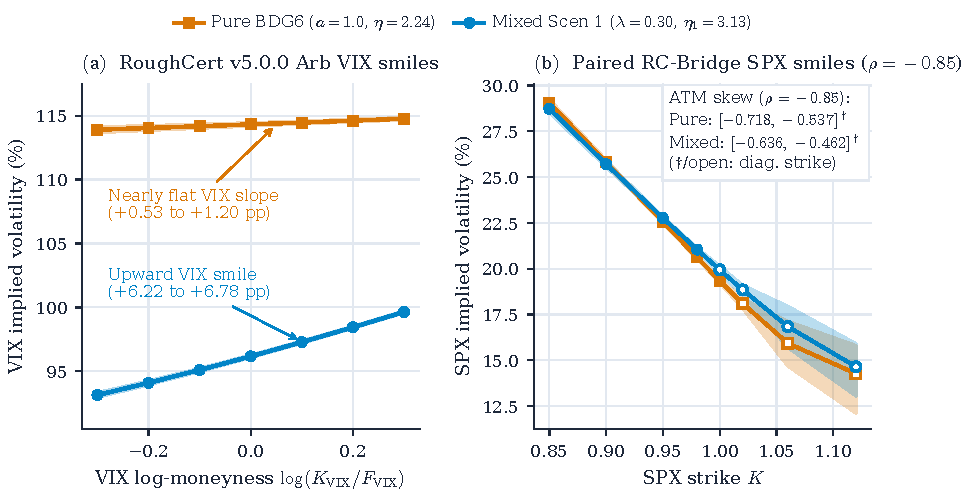
\includegraphics[width=\textwidth]{figures/fig_e6_joint_spx_vix.pdf}
  \caption{Joint SPX--VIX audit at $H=0.10$, $T=0.25$, $\xi_0=0.235^2$. (a) Arb-certified VIX smiles from \RoughCert{} \CompanionTag{} for Pure~BDG6 and Mixed~Scen.~1. (b) $65{,}536$-path \RCBridge{} SPX smiles at $\rho=-0.85$ (filled: asymptotic envelope; open: diagnostic).}
  \label{fig:e6_joint}
\end{figure}

Four conclusions follow, each with its epistemic status.
\begin{itemize}
  \item \emph{A certified VIX lift beside statistically controlled SPX skews.} At $\rho=-0.70$, where all three stencil strikes $\{e^{-0.02},1,e^{0.02}\}$ have asymptotic-envelope status for both models, Pure~BDG6 pairs a nearly flat Arb-certified VIX slope of $[\ESixPureVixSlopeLo,\ESixPureVixSlopeHi]\,\mathrm{pp}$ with an SPX ATM skew of $[\ESixPureSeventySkewLo,\ESixPureSeventySkewHi]$, whereas Mixed~Scen.~1 raises the VIX slope to $[\ESixMixVixSlopeLo,\ESixMixVixSlopeHi]\,\mathrm{pp}$ and keeps a steep SPX skew of $[\ESixMixSeventySkewLo,\ESixMixSeventySkewHi]$. The two certified VIX intervals are separated by at least $\ESixVixLiftLo\,\mathrm{pp}$, so the VIX lift is a property of the continuum models rather than a discretisation artefact; the SPX skews carry asymptotic-envelope guarantees with joint coverage at least $0.90$. At $\rho=-0.85$ (Figure~\ref{fig:e6_joint}(b)) the skews steepen to $[\ESixPureSkewLo,\ESixPureSkewHi]^\dagger$ (Pure~BDG6) and $[\ESixMixSkewLo,\ESixMixSkewHi]^\dagger$ (Mixed~Scen.~1), where the daggers mark diagnostic flags on the stencil.
  \item \emph{Refinement of the $\rho=-0.85$ stencils.} With one more level ($n_L=\RefFinestLevel$) and fresh seeds (Supplementary Table~S1), the Mixed~Scen.~1 stencil reaches asymptotic-envelope status and its skew interval narrows to $[\RefMixSkewLo,\RefMixSkewHi]$; only the call wing $K=1.06$ remains diagnostic. For Pure~BDG6 the skew interval becomes $[\RefPureSkewLo,\RefPureSkewHi]$, but the stencil stays flagged: at $K=1$ and $K=e^{0.02}$ the finest increment is resolved while the previous one is not (an emerging increment), and $K=1.06$ contracts too slowly.
  \item \emph{Coarse-grid skew estimates carry no bias control.} For Mixed~Scen.~1 at $\rho=-0.85$, a single-grid left-point simulation with $n=64$ gives an ATM skew point estimate of $\ESixMixCoarseSkew$. It falls inside the diagnostic bracket, but a single grid gives no estimate of its own discretisation bias, whereas \RCBridge{} reports the residual uncertainty together with the contraction warning.
  \item \emph{Stress test of the contraction gate.} Across the nine model--correlation rows ($\ESixStrikesTotal$ strike evaluations), \RCBridge{} reports no diagnostic strike for Pure~E14 at $\rho\in\{-0.85,-0.90\}$ and Pure~BDG6 at $\rho=-0.95$, and flags $\ESixTotalDiag$ strikes in total: $\ESixMixDiagHighRho$ of them in Mixed~Scen.~1 ($\eta_1=3.1305$) at $|\rho|\ge 0.85$ and $\ESixMixDiagAll$ in Mixed~Scen.~1 overall, where heavy variance tails slow the dyadic contraction. Theorem~\ref{thm:bridge_envelope}(iii) flags these strikes instead of certifying slow contraction, which tells a validator where finer grids or larger budgets are needed; the refinement above shows what one more level achieves for the two $\rho=-0.85$ rows.
\end{itemize}

\FloatBarrier
